\section{Auswertung}
\label{sec:Auswertung}
Zunächst werden die Messwerte der Auslenkung gegen die Ablenkspannung aufgetragen und mithilfe einer linearen ausgleichsrechnung approximiert
 \begin{figure}
     \centering
     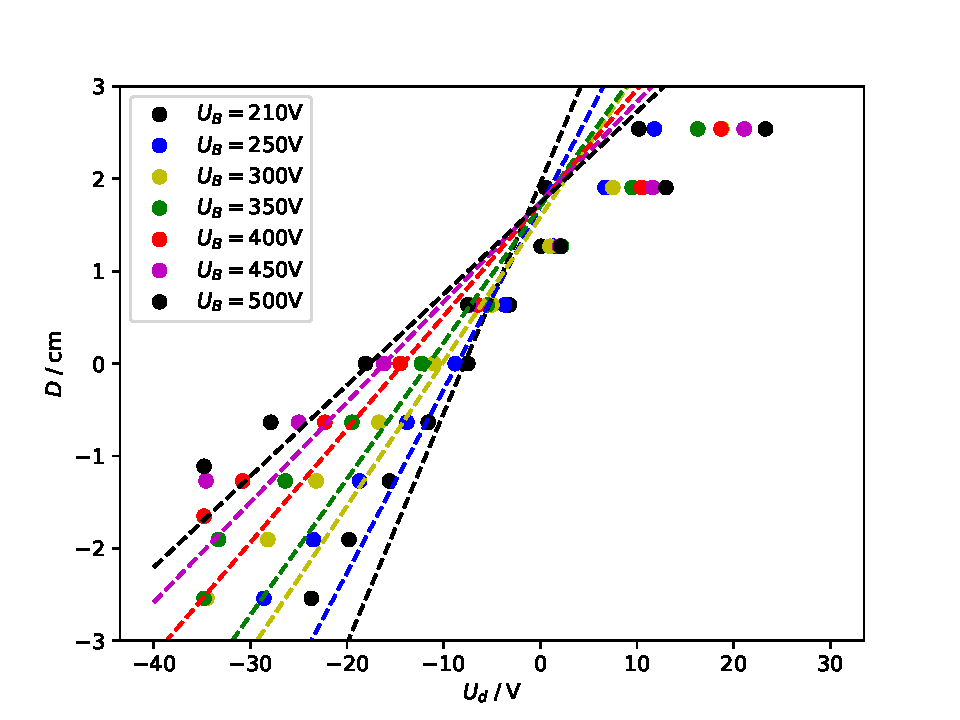
\includegraphics[width = 0.7\textwidth]{plots/all.pdf}
     \caption{Die Messwerte der Auslenkung D werden gegen die Beschleunigungsspannung $U_d$ aufgetragen.
              Mit einer linearen Ausgleichsrechnung wird der Verlauf der Werte approximiert.}
 \end{figure}
Mit dem linearen Ausgleich ergibt sich nach,
\begin{align}
    D(U_d) = m\cdot U_d + b  \nonumber \\
\end{align}

die Empfindlichkeit E der Braunschen Röhre mit
\begin{equation}
    E(U_d)=\frac{D}{U_d}=m.
\end{equation}

\begin{table}
    \centering
    \begin{tabular}{c | c c c c c c c}
        \toprule
        $U_B\;/\;V$&210&250&300&350&400&450&500\\
        \midrule
        Empfindlichkeit $E\;/\;\frac{cm}{V}$& 0.2491& 0.1473& 0.1563& 0.1473& 0.1225& 0.1083& 0.0985\\
        \bottomrule
    \end{tabular}
    \caption{}
\end{table}
\newpage
Für die Bestimmung der Apperaturkonstanten $K$, wird zunächst der Kehrwert der Beschleunigungsspannung $U_B$
gegen die Empfindlichkeit $E$ aufgetragen. Mithilfe einer Linearen Asugleichsgeraden, der Form
\begin{equation}
    E(1/U_b) = a\cdot \frac{1}{U_b} + b  \nonumber
\end{equation}
\begin{figure}
    \centering
    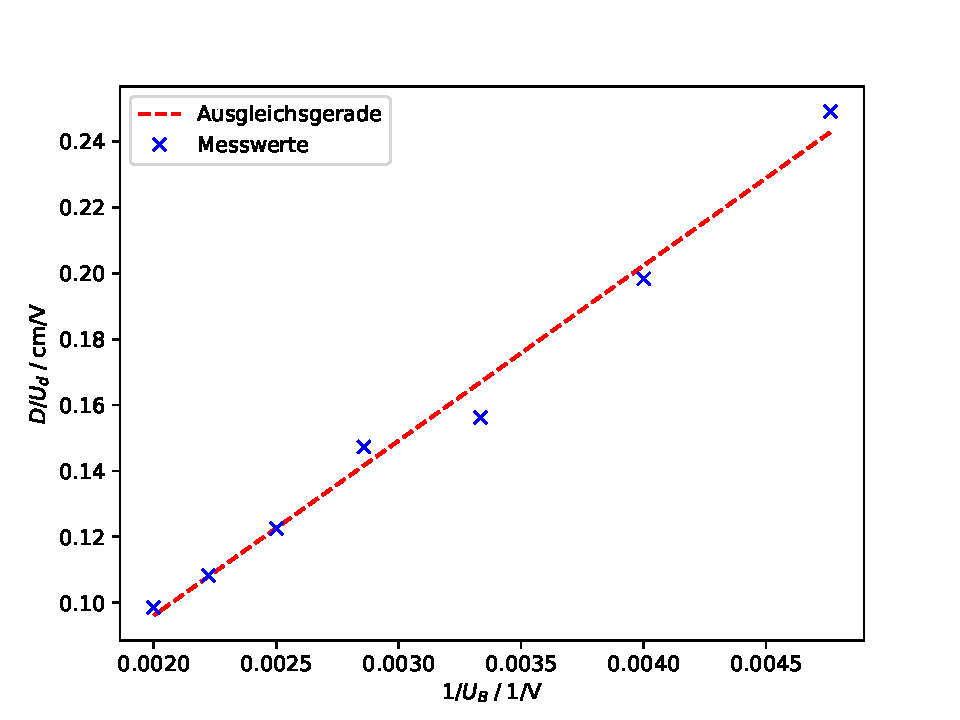
\includegraphics[width=0.8\textwidth]{plots/all2.pdf}
    \caption{}
\end{figure}
mit den Parametern,
\begin{align}
    a&=(53.13\pm2.62),\\
    b&=(-0.01\pm0.0085).
\end{align}
Es zeigt sich, dass der y-Achsenabschnitt hinreichend klein ist, sodass er für folgende Rechnung vernachlässigt wird.\\

Somit folgt aus der Beziehung
\begin{align}
    D&=\frac{p}{2d}L\frac{U_d}{U_B}\\
    \frac{D}{U_d}&=\frac{Lp}{2d} \cdot \frac{1}{U_B}=a\cdot \frac{1}{U_B}
\end{align}
\begin{align}
    p = 1.9\text{cm} \\
    d = 0.38\text{cm}\\
    L = 14.3\text{cm}\\
    \frac{pL}{2d} =35.75\text{cm} \\
    a = (53.13\pm2.62)\text{cm}\\
    \textrm{abs. Abweichung} = \\
    \textrm{rel. Abweichung} = \\
\end{align}
